\documentclass[11pt]{report}

% ----------------------------------------------------

\usepackage[T1]{fontenc}
\usepackage[margin=2cm, top=2cm, includefoot]{geometry}
\usepackage{graphicx}
\usepackage{float}
\usepackage{xcolor}
\usepackage{listingsutf8}
\usepackage{realboxes}
\usepackage{framed}
\usepackage{titlesec}
\usepackage{tabto}
\usepackage{url}
\usepackage{csquotes}
\usepackage{chngcntr} \counterwithout{figure}{chapter}
\usepackage[hidelinks]{hyperref}
\usepackage{parskip}
\usepackage[most]{tcolorbox}
\usepackage{fancyhdr}
\usepackage{tabularx}
\usepackage{sectsty}
\usepackage{afterpage}
\usepackage{amsmath}
\usepackage{amssymb}
\usepackage{amsthm}

\usepackage[french]{babel}
\usepackage{blindtext}
\usepackage{enumitem}
\newtheorem{theorem}{Theoreme}

\definecolor{dkgreen}{rgb}{0,0.6,0}
\definecolor{gray}{rgb}{0.5,0.5,0.5}
\definecolor{mauve}{rgb}{0.58,0,0.82}

\lstset{frame=tb,
  inputencoding=utf8/latin1,
  language=Python,
  aboveskip=3mm,
  belowskip=3mm,
  showstringspaces=false,
  columns=flexible,
  basicstyle={\small\ttfamily},
  numbers=none,
  numberstyle=\tiny\color{gray},
  keywordstyle=\color{blue},
  commentstyle=\color{dkgreen},
  stringstyle=\color{mauve},
  breaklines=true,
  breakatwhitespace=true,
  tabsize=3
}

% ----------------------------------------------------

\graphicspath{{figs/}{../}}

\setlength{\headheight}{40pt}
\pagestyle{fancy}
\fancyhf{}

\renewcommand{\headrulewidth}{3pt}
\renewcommand{\headrule}{\hbox to\headwidth{\color{black}\leaders\hrule height \headrulewidth\hfill}}

\titleformat{\chapter}[display]{\normalfont\centering\bfseries}{\vspace{-100pt}}{0pt}{\Huge}
\titleformat{\section}{\normalfont\scshape}{1em}{\thesection}{\Large}

% ----------------------------------------------------

\title{Modèle épidémie SIR en épidémiologie : présentation et illustration}
\author{TURPIN Yohann, GEHU Lauric, FOSSET Jaurel}


% ----------------------------------------------------

\begin{document}
    \cfoot{\thepage}
    
    \makeatletter
    \begin{titlepage}
        \reversemarginpar\marginpar
        {
            \vspace{-86pt}
            \hspace*{25pt}
            
\includegraphics{logo_esirem.png}
        }
        
        {\centering
            \vspace{3cm}
            \par\vspace{5cm}
            {\scshape\huge\textbf{\hspace{2cm}\@title}} \par\vspace{6cm}
            
            {\LARGE
            \begin{flushright}
                    \item \@author
                    \item \today
            \end{flushright}
            }
        }
    \end{titlepage}
    \makeatother


    \null
    \thispagestyle{empty}
    \addtocounter{page}{-1}
  
    
    \tableofcontents
    \newpage

    \setlength{\abovedisplayskip}{6pt}
    \setlength{\belowdisplayskip}{6pt}


    %%% PUBLICATIONS QUE VOUS SOUHAITEZ FAIRE APPARAITRE SANS LES CITER

%Int Journal
\nocite{HKC16}
\nocite{THV14}
\nocite{HKCMST12}
%Int Conf
\nocite{FRT16a}
\nocite{FRT16}
\nocite{FRT16f}
\nocite{HdT15a}
\nocite{HdT15}
\nocite{CDR12}
\nocite{HKC12}
\nocite{CAT11a}
\nocite{CAT11b}
\nocite{wise2011}
\nocite{AAC08a}
\nocite{TDL07}
\nocite{TD07}
\nocite{DT07}
\nocite{TDL07a}
\nocite{TD07a}
%Book Chapter
\nocite{Tra12}
\nocite{mTX09}
%National Journal
\nocite{FRT16b}
\nocite{HKC13}
\nocite{CAC12}
%National Conference
\nocite{HDT13}
\nocite{CDRa12}
\nocite{HKCa12}
\nocite{CAT11}
\nocite{HTVa11}
\nocite{CATV10}
\nocite{ACT10}

    \newpage

\section*{Remerciements}
Nous tenons à exprimer notre profonde gratitude à l’enseignante Karine Serrier pour son soutien, ses conseils et sa patience tout au long de la réalisation de ce rapport.Nous sommes reconnaissants de l’avoir eu comme encadrante et nous espérons que sa passion des mathématiques et sa bonne humeur se ressentiront dans le travail fourni.


    \section{Introduction}

\begin{frame}
 	 \frametitle{Contextualisation}
	\begin{itemize}
			\item Crise du COVID-19
			\item Evolution
			\item Pression hospitalière
	\end{itemize}
\end{frame}


\begin{frame}
    \frametitle{Problématique}
	De quelle façon les entités sanitaires parviennent-elles à nous partager des résultats ?
\end{frame}


\begin{frame}
    \frametitle{Outils à disposition}

    \begin{block}{Modèles déterministes}
        Régis par des hypothèses simplificatrices ne traduisant pas la réalité.
    \end{block}


    \begin{block}{Modèles stochastiques}
        Calculs plus complexes mais prenant en comptant les phénomènes aléatoires.

    \end{block}
\end{frame}

\begin{frame}
    \frametitle{Objectifs}
     \begin{itemize}
    	\item Vérifier les modèles
	\item Déterminer une condition d'équivalence entre ces modèles 
     \end{itemize}
\end{frame}




    \chapter{Modèles déterministe}

\begin{frame}
        \frametitle{Modéle SIR}

        \begin{block}{Définition}

                Modéle divisé en trois groupe :
                \begin{itemize}
                        \item Susceptible : personnes saines qui n'ont pas encore contracté la maladie
                        \item Infectés : les malades qui transemettent activement la maladie
                        \item Rétablis : les guéris ou mort, qui ne peuvent plus contracté la maladie.
                \end{itemize}

        \end{block}
\end{frame}

\begin{frame}
        \frametitle{Modéle SIR}

        \begin{alertblock}{Equation}

                $$ \frac{dS}{dt} = -\frac{\beta SI}{N} \qquad \frac{dI}{dt} = \frac{\beta SI}{N} - \gamma I \qquad \frac{dR}{dt} = \gamma I $$

                \begin{itemize}
                        \item $N$ : taille totale de la population
                        \item $\beta$ : taux de contact
                        \item $\gamma$ : taux de guérison.
                \end{itemize}

        \end{alertblock}
\end{frame}

\begin{frame}
        \frametitle{Nombre de reproduction de base ($R_0$)}

        \begin{block}{Définition}
                Nombre attendu d’infections générées par un individu infectieux dans une grande population susceptible.
        \end{block}

        \begin{alertblock}{SIR}
                $$ R_0 =  \lambda i $$
                \begin{itemize}
                        \item $i$ : durée moyenne de la période infectieuse
                        \item $\lambda$ : intensité du processus de Poisson homogène qui modélise les contacts entre les individus infectés et les individus susceptibles
                \end{itemize}
        \end{alertblock}
\end{frame}


    \section{Les modèles stochastiques}

\section{Reed et Forst}

Le modèle SIR dans l’état que nous avons donné, possède certaines incohérence vis à vis
de la réalité. En effet, il suppose que chaque individu de la population a une chance égale d'entrer
en contact avec tous les autres individus, et que la chance de propager l’épidémie est, elle aussi uniforme.
C’est ici qu’intervient le modèle stochastique de Reed et Frost présenté en 1928, qui redéfinit le
modèele cité précedemment. S'ils sont infectés, ils deviennent d'abord infectieux pendant un certain
temps, puis se rétablissent et deviennent immunisés. Le modèle est généralement utilisé avec une
dynamique à temps discret, où la période infectieuse est courte et précédée d'une période de latence
plus longue. Les nouvelles infections se produisent par génération, séparées par la période de
latence. Les probabilités dans chaque génération dépendent de l'état de l'épidémie dans la
génération précédente, et sont spécifiées par des probabilités binomiales.

\begin{align}
P(Y_{j+1} = y_{j+1} | X_0 = x_0, Y_0 = y_0, ..., X_j = x_j, Y_j = y_j) &= P(Y_{j+1} = y_{j+1} | X_j = x_j, Y_j = y_j) \\
&= \binom{x_j}{y_{j+1}}(1 - q^{y_j})^{y_{j+1}}(q^{y_j})^{x_j - y_{j+1}}
\end{align}

\subsection{Loi Binomiale}

Une variable aléatoire X suit une loi de poisson si :
$$ P(X = k) = \binom{n}{k}p^k(1 - p)^{n-k} $$
La loi Binomiale est la loi suivis par la variable aléatoire X qui compte le nombre de succés de n expériences de Bernouli consécutives et indépendantes.
La loi de Bernouli est la loi suivis par l'expérience qui peut résussir avec une probabilités p.



\subsection{Bartlett}

\begin{frame}
    \frametitle{Bartlett}

    \begin{block}{Définition du Modéle}
        Au temps initial, la population se compose de m infectés et n susceptibles. Chaque infecté a une période de contagion qui suit une loi I (moyenne $i$ variance $\sigma^2$) indépendante de celle des autres. Et pendant cette période il rencontre un autre individu donné suivant les instants de saut d’un processus de Poisson d’intensité $\frac{\lambda}{n}$.
    \end{block}

    \begin{itemize}
        \item Ainsi, pendant un temps $dt$, la probabilité qu’un infecté rencontre un individu initialement susceptible vaut $\lambda$.
        \item On appellera $E_{n,m}(\lambda, I)$ une telle épidémie.
        \item $R_0 = \lambda i$ décideras si l'épidémie deviendra une pandémie ou endémie.
    \end{itemize}

\end{frame}

\begin{frame}
    \frametitle{Loi de poisson}

    \begin{block}{Définition}
        Une variable aléatoire X suit une loi de poisson si :
        $$ P(X=k) = \exp(-\lambda \frac{\lambda^k}{k!}) $$
    \end{block}

    \begin{itemize}
        \item Cette loi est dite des événements rares : elle est souvent utilisé pour modéliser le nombre d'occurences d'un phénoménes dans un temps donnés, le phénoméne devant étre rare dans un temps court.
    \end{itemize}

\end{frame}

\section{La construction de Selke}

Une construction équivalente, proposée par Sellke en 1983, se base sur l’idée d’affecter à chaque individu une capacité de résistance à l’épidémie et de définir, à partir du nombre d’infectés, une pression de l’épidémie et un critère d’infection sur la résistance de l’individu. Pour y arriver, les chaînes de Markov sont utilisées pour modéliser l’évolution de l’épidémie au fil du temps, en prenant en compte les transitions entre les différents états de l’épidémie (susceptible, infecté, rétabli). Les processus de Poisson sont utilisés pour modéliser le nombre d’infections qui se produisent dans un intervalle de temps donné, en supposant que les infections se produisent de manière aléatoire et indépendante les unes des autres.

De plus cette construction permet aussi d’identifier un paramètre important quand il s’agit de modéliser une épidémie : sa taille finale. Ici, l’expression de la taille finale de l’épidémie dépend du nombre de reproductions de base $R_0$, qui est le nombre moyen de personnes qu’un individu infecté infecte au début de l’épidémie. Plus le nombre de reproductions de base est élevé, plus la taille finale de l’épidémie sera grande. L’expression de la taille finale de l’épidémie peut être calculée à partir de l’équation $1 - \tau = e - R_0\tau$, où $\tau$ est la proportion de la population qui sera infectée à la fin de l’épidémie .


\subsection{Chaine de Markov}

Une chaîne de Markov est un processus aléatoire à temps discret dont la principale caractéristique est l’absence de mémoire et l’existence de probabilités de transition entre les états de la chaîne. Cela signifie que seul l’état actuel du processus a une influence sur l’état qui va suivre.

En considérant S un ensemble fini (ou dénombrable) et $(X_n)_{n \in \mathbb{N}}$ une suite de variables aléatoires définie sur le même univers $\Omega$ munit de la mesure de probabilité $\mathbb{P}$ et à valeurs dans S. $(X_n)$ chaîne de Markov homogéne si :

\begin{itemize}
    \item \textbf{Propriété de Markov} : $\forall n \in \mathbb{N}$ et $(x_i)^n \in S^n (i \in [[0, n+1]])$ \\
    $$ \mathbb{P}(X_{n+1} = x_{n+1} | X_{0:n} = x_{0:n}) = \mathbb{P}(X_{n+1} = x_{n+1} | X_n = x_n) $$
    \item \textbf{Homogénéité} : $\mathbb{P}(X_{n+1} = y | X_n = x)$ ne dépend pas de n, $\forall (x, y) \in S^2$. On note alors $p(x, y)$ cette probabilité.
\end{itemize}

La loi de $X_0$ est appelée loi initiale de la chaîne de Markov, $P = (p(x, y))_{x,y \in S}$ est appelée matrice de transition.

\subsection{Processus de Poisson}



\section{Que fait-on du début de l'épidémie}


    \chapter{Conclusion}

\begin{theorem}[Loi faible des grands nombres]
 Soit $(X_n)_{n \in \boldsymbol{N}}$ une suite de variable aléatoire indépendante et identiquement distribuée de même loi que X (loi mère). Si $\mathbb{E}[|X|] < +\infty$, alors $\overline{X_n} \rightarrow \mathbb{E}[X]$
\end{theorem}


On ne rappele pas la loi faibles des grands nombres pour rien.\\
En effet,elle peut être observée dans les modèles SIR déterministes et stochastiques.\\
Plus précisément,on peut montrer le modèle stochastique converge vers le modèle déterministe correspondant lorsque la taille de la population tend vers l'infini. Ainsi,on peut en conclure que la faible loi des grands nombres est un concept qui fournit une justification mathématique à l'utilisation de modèles déterministes pour approcher le comportement des modèles stochastiques parmi une grande population, tel que pendant une épidémie mondiale.

\begin{figure}[h]
\centering
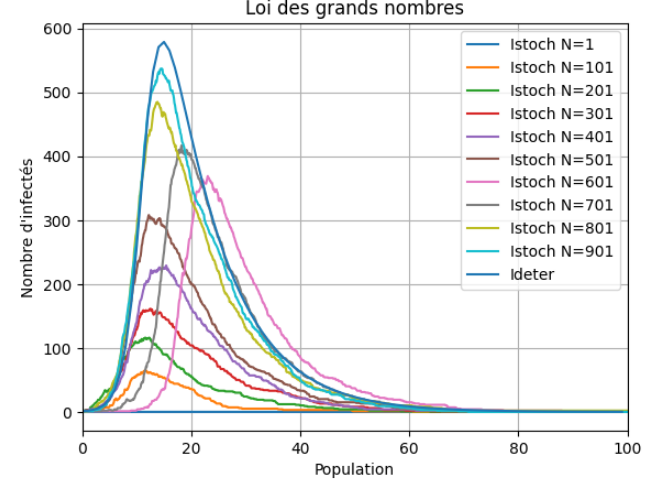
\includegraphics[width=0.5\textwidth]{figs/sir_loi_grands_nombres.png}
\caption{Loi des grands nombres appliqués au modèle stochastique SIR}
\label{fig:loi_grands_nombres}
\end{figure}


    \listoffigures
    \listoftables

	\chapter{Annexes}
\begin{appendix}
\section{Simulation du modèle déterministe}
\label{simu_det}
\lstinputlisting[language=Python]{sir_deterministe.py}
\section{Simulation du modèle stochastique}
\lstinputlisting[language=Python]{sir_stochastique.py}
\end{appendix}


	
    \renewcommand{\bibname}{Bibliographie}
    \bibliographystyle{alpha}
    \begin{thebibliography}{99} % Vous pouvez ajuster le nombre maximal d'étiquettes
    \addto\captionsfrench{\renewcommand{\refname}{Bibliographie}}
	\bibitem{source1}
	Pierre24
	\emph{Modéliser une épidémie}.\\
	\url{https://zestedesavoir.com/tutoriels/3790/modeliser-une-epidemie/}
	
	\bibitem{source2}
	Manon Costa
	\emph{Modélisation stochastique d’une épidémie SIR}.\\
	\url{https://www.math.ens.psl.eu/shared-files/10744/?introduction%20au%20domaine%20de%20recherche.pdf}
	
	
	\bibitem{source3}
	Tom Britton,Etienne Pardoux
	\emph{Stochastic epidemics in a homogeneous community}.\\
	\url{https://www.i2m.univ-amu.fr/perso/etienne.pardoux/_media/tb-ep_homogenepid.pdf}
	
	\bibitem{source4}
	H. Andersson, T. Britton
	\emph{Stochastic Epidemic Models and their Statistical Analysis. Lecture Notes in Statistics, Springer Verlag, 2000.}.\\
	\url{https://sci-hub.3800808.com/10.1007/978-1-4612-1158-7}





	% Ajoutez d'autres entrées de bibliographie au besoin

	\end{thebibliography}


\end{document}
